\documentclass[tikz]{standalone}
\usepackage{ifthen}
\renewcommand\familydefault{\sfdefault}
\usepackage{tikz}
\usetikzlibrary{calc}
\def\pixels{
{0,2,0,0},
{0,8,0,4},
{2,2,4,16},
{8,16,128,2},
}

% Font color for 2 and 4: #776e65
% Font color for rest: #f9f6f2
% Grid color: #bbada0
% Font family: "Clear Sans", "Helvetica Neue", Arial, sans-serif

\definecolor{pixel 0}{HTML}{CCC0B3}
\definecolor{pixel 2}{HTML}{EEE4DA}
\definecolor{pixel 4}{HTML}{EEE4DA}
\definecolor{pixel 8}{HTML}{F2B179}
\definecolor{pixel 16}{HTML}{F59563}
\definecolor{pixel 32}{HTML}{F2B179} % TODO
\definecolor{pixel 64}{HTML}{F2B179}
\definecolor{pixel 128}{HTML}{EDCF72}
\definecolor{pixel 256}{HTML}{F2B179} % TODO
\definecolor{pixel 512}{HTML}{F2B179} % TODO
\definecolor{pixel 1024}{HTML}{F2B179} % TODO
\definecolor{pixel 2048}{HTML}{F2B179} % TODO
\definecolor{pixel 4096}{HTML}{F2B179} % TODO
\begin{document}
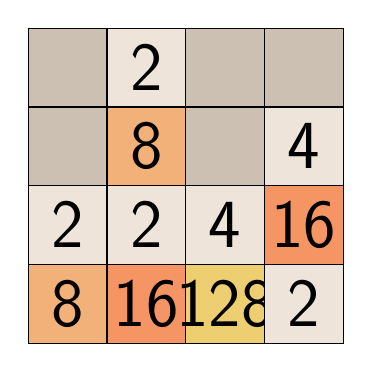
\begin{tikzpicture}
  \foreach \line [count=\y] in \pixels {
    \foreach \pix [count=\x] in \line {
      \draw[fill=pixel \pix] (\x,-\y) rectangle +(1,1);
      
      \ifthenelse{\equal{0}{\pix}}
           {}
           {\node at ($(\x,-\y) + (0.5,0.5)$)    {\Huge \pix};}
    }
  }

\end{tikzpicture}
\end{document}
